\chapter{Basic Commands}
\section{Defining the Basic Geometry of Calculation}
To define the basic geometry type of calculation, the command
\begin{xmllisting} 
<domain geometryType="plane">
...
</domain
\end{xmllisting} 
is used. Allowed parameters for {\bf type} are
{\bf 
\begin{itemize}
\item \xatv{plane}
\item \xatv{axi}
\item \xatv{3d}
\end{itemize}}

If needed, a more detailed description of the geometry type must be
provided in the individual PDEs (e.g. in \xel{mechanics}: \xatv{planeStrain}).



\section{Defining the Input and Output File Format}
\subsection{Input File}
The input file defines the mesh with its nodes, elements and regions. You can
set the input file on
the command line via the \textbf{-m} option or define it within the problem file
itself as described below.

The following example uses the HDF5 format and HDF5 specific option that
linearizes the mesh (for for the non-matching grid technique).
\begin{xmllisting} 
<input>
  <hdf5 fileName="coupled.h5" linearizeEntities="iface_1 iface_2" />
</input>
\end{xmllisting}

The file input formats are
  
\begin{xellist}{Availabe \xel{output} formats}
\xel{mesh} & & ASCII format specific for CFS++ to be generated by GiD and
               ANSYS \\
\xel{hdf5} & & Compact binary format specific for CFS++. To generated from
               \textit{mesh} by \textbf{cfstool} \\
\xel{unv} &  & Legacy format only
\end{xellist}

\begin{xellist}{Available \xel{input} formats}
\\
\end{xellist}

\subsection{Output File}
Ouput can be written to different output formats simultaneously. Most formats
write into a adjustable subdirectory, with the defaults listed in the table
below. The column \textit{Single} expresses if the format writes multiple
timesteps/ frequencies/ iterations into a single file or creates seperate files.
The advantage for the later is, that one can visualize intermediate results. The
most important formats are \textit{hdf5, gid} and \textit{text}. The formats
\textit{rst} and \textit{unv} have no relevance.

\medskip

\begin{tabular}{llll} 
\toprule \rowcolor{darkgrey}
Output & Target dir & Single & Description  \\
\midrule
\xel{hdf5} & 'results\_hdf5' & yes & To be visualized with ParaView via CFS
reader plugin \\
\xel{gid} & 'results\_hdf5' & yes & For GiD, has attribute \textit{binaryFormat}
\\
\xel{text} & 'history' & no & Writes tabular ASCII for gnuplot, MATLAB, \ldots
\\
\midrule 
\xel{gmv} & 'simoutput\_gmv' & no & Free, fast but difficult to use ``general
mesh viewer'' \\
\xel{info} & - & yes & toggle history output to \textit{info.xml} file \\
\midrule
\xel{rst} & ? & ? & ANSYS format, rarely used \\
\xel{unv} & ? & ? & Legacy format only \\
\bottomrule
\end{tabular}

\medskip

All formats but \xml{text} are for the visualization of node and element values
based on the mesh information.

All formats have implicitly the \xml{id} attribute set to a string with the
format name. 

\subsubsection{\xel{gid}}
The following options are available
\begin{xatlist}{Format options for \xel{gid}}
\xat{binayFormat} & \xatv{yes}, \xatv{no} & See below, default
is \xatv{yes} \\ 
\xat{directory} & \textit{directory} & See below, default is
``results\_gid''
\end{xatlist}
The binary format writes a single file ``\textit{problem}.post.bin''. In the
non-binary file two ASCII files
``\textit{problem}.post.msh'' and ``\textit{problem}.post.res'' are created. 

If the \xat{directory} attribute is set to ``.'' the current directory
is used.

\subsubsection{\xel{hdf5}}
The Hierarchical Data Format (5) is a standard format for simulation data.
There are various tools for conversion and visualization available (e.g
hdfview). MATLAB can also read and write HDF5 files. Furthermore HDF5 files
can converted into gid files via the cfstool.

Additional information is stored, like the problem XML file and history data.

The HDF5 files can be visualized via ParaView by the CFS-HDF5 reader.

The mesh within a HDF5 file can be used as input for a CFS simulation.

\begin{xatlist}{Attributes of the \xel{hdf5} element}
\xat{directory} & \textit{directory} & See \xel{gid}, default is
``results\_hdf5'' \\ 
\xat{compressionLevel} & \textit{1 \ldots 9} & has not much effect \\
\xat{maxChungSize} & \textit{number} & ??? \\
\xat{externalFiles} &  \xatv{yes}, \xatv{no} & ??? 
\end{xatlist}

\subsubsection{\xel{text}}
The \xel{text} element writes the following data:
\begin{itemize}
  \item nodes named by \xel{nodeList} within \xel{nodeResult}
  \item elements named by \xel{elementList} within \xel{elementResult}
  \item integral \xel{regionResult} and \xel{surfRegionResult} results
\end{itemize}

The same information can also be found in the \textit{info.xml} file.

\begin{xatlist}{Attributes of the \xel{text} element, only for special cases.}
\xat{commentChar} & \xatv{\#}, \xatv{\%}, \ldots & gnuplot
(\#), matlab
(\%), \ldots \\ 
\xat{fileCollect} & \xatv{timeFreq}, \xatv{entity},
\xatv{altogether} & triggers new files \\ 
\xat{coordSysId} & \xatv{own-id} & see below \\
\xat{entityNumbering} & \xatv{global}, \xatv{consecutive} &
                      see below \\

\bottomrule
\end{xatlist}

When \xat{fileCollect} is set to \xatv{timeFreq} for every
timestep/frequency step a new result
file is created. Together with the \xat{coordSysId} does this allow to
create acoustic directivity
patterns.

The \xat{entityNumbering} attribute determines, how the names of files are
determined: In case of \xat{fileCollect} = \xatv{entity} (default), the node /
element number enters the name of the history text file. If \xatv{global}
numbering is selected (default), the global node / element number is taken. In
case of \xatv{consecutive}, a local, 1-based numbering for every node / element
list is taken. This is advantageous, if the history files should have the same
name, independent of the mesh discretization, where the global node numbers
change.

\subsubsection{\xel{info}}
Writes the same node, element and integral data as the \xel{text} writer.
The data is written to the \textit{info.xml} output file. The xml data can be
filtered and converted to xml, text, html, \ldots
via XSLT-stylesheets. Examples can be found within the cfs code.  
% \begin{center}
% \begin{tabular}{lll}
% \toprule 
% Attribute & Values & Description \\
% \midrule
% output & \xml{true}, \xml{false} & toggle history output to \textit{info.xml}
\\
% \bottomrule
% \end{tabular} \\[0.5ex]
% Attributes of the \xml{info} element, only for special cases.
% \end{center}
\section{Material Data File}
To specify the name of the material file, the command 
\begin{xmllisting}
<fileFormats>
...
	<materialData file="mat.xml" format="xml"/>
</fileFormats>
\end{xmllisting}
must be used. The default name for the material file is {\bf mat.xml}.




% =============================================================================
% TYPES OF ANALYSIS
% =============================================================================
%
\section{Analysis Techniques}\label{subsec:Analysis}
In the config-file, the actual analyis type is defined by a sub element
within the analyis element, the following example shows the simplest case - a
static analysis:
\begin{xmllisting}
<sequenceStep>
  <analysis> 
    <static/>
  </analysis>
  ..
\end{xmllisting}
\noindent
The availabel analys types are one of
\begin{itemize} 
\item \xel{static} 
\item \xel{harmonic}
\item \xel{transient}
\item \xel{eigenFrequency}
\item \xel{paramIdent}
\item \xel{multiSequence}
\end{itemize}


% ----------------------------------------------------------------------------
\subsection{Static Analysis}
% ----------------------------------------------------------------------------
%
%
For static analysis, no additional information beside the element
\xelempty{static} is needed. See also the example above.

% ----------------------------------------------------------------------------
\subsection{Transient Analysis}
% ----------------------------------------------------------------------------
%
For a transient analysis the following block is mandatory:
\begin{xmllisting}
<transient>
  <numSteps>20</numSteps>
  <deltaT>1e-3</deltaT>
</transient>
\end{xmllisting}
Optional parameters are:
\begin{xmllisting}
<writeRestartInc>5</writeRestartInc>
\end{xmllisting}
\noindent
Herein, the different tags have the following meaning:\\
\begin{xellist}{Parameters for \xel{transient} element}
\xel{numSteps}   & \xparam{numSteps} &  number of time steps\\
\xel{deltaT}    & &  time step size in seconds\\
\xel{writeRestartInc} &&  step increment for writing a restart
 file (currently only for mechanic PDE)
\end{xellist}

\bigskip

\noindent
For simple excitations (ramps, dirac impulse, sin, \ldots) one might
consider using a mathematical expression in a boundary condition as
shown in the following example: A mechanical system is excitated with a
rectangle aproximating a dirac impuls.   
\begin{displaymath}
z = \left\{ \begin{array}{ll}
1 & \textrm{if $t \in [0.001; 0.002]$}\\
0 & \textrm{else}\\
\end{array} \right.
\end{displaymath}
\begin{xmllisting} 
<sequenceStep>
 <analysis>
  <transient>
    <numSteps>30</numSteps>
    <deltaT>1e-4</deltaT>
  </transient>
 </analysis>
 <pdeList>
  <mechanic ..>
   <bcsAndLoads>
     ..
     <load name="load" dof="z" value="if(t lt 0.001 or t gt 0.002,0.0,1.0)"/>
     ..
   </bcsAndLoads>
  </mechanic>
 </pdeList>
</sequenceStep>
\end{xmllisting}

\noindent
For more complex time signals use \xel{timeDataFile} with the following
column oriented
structure:
\begin{verbatim}
timeVal1          funcVal1
timeVal2          funcVal2
timeVal3          funcVal3
...
\end{verbatim}

% ----------------------------------------------------------------------------
\subsection{Harmonic Analysis}
% ----------------------------------------------------------------------------
%
Specification of parameters for a \xel{harmonic} analysis is done by adding
a \xel{harmonic} section to the parameter file. When all currently
available
parameters are set this section takes the following form:
%
%
\begin{xmllisting}
  <harmonic>
    <numFreq>    100   </numFreq>
    <startFreq>  50   </startFreq>
    <stopFreq>   1000   </stopFreq>
    <sampling>   log   </sampling>
  </harmonic>
\end{xmllisting}
%
%
The meaning for the parameters are given in the following table
%
%

\begin{xellist}{Parameters for \xel{harmonic} element}
\xel{numFreq} & $\nat$ & specifies the number $N$ of frequencies for which
                   a simulation is to be performed\\
\midrule
\xel{startFreq} & $> 0$ & sets $f_1$, i.e. the smallest frequency for which a
                    simulation is to be performed\\
\midrule
\xel{stopFreq} & $\geqslant$ startFreq & sets $f_N$, i.e. the largest frequency
for
                                   which a simulation is to be performed\\
\midrule
\xel{sampling} & linear & in this case a linear sampling of the interval
                    $[f_1,f_N]$ is performed, i.e.
                    \begin{displaymath}
                   f_k = f_1 + (k-1) \frac{f_N - f_1}{N-1}
                   \enspace,\mbox{ for } k = 1,\ldots,N
                   \end{displaymath} \\
               
 
         & log    & in this case a logarithmic sampling of the interval
                    $[f_1,f_N]$ is performed, i.e.
                    \begin{displaymath}
                    f_k = f_1 \cdot
                    \left(\frac{f_N}{f_1}\right)^{\frac{k-1}{N-1}}
                   \enspace,\mbox{ for } k = 1,\ldots,N
                    \end{displaymath}
                    This leads to a finer sampling at the beginnig of the
                    interval and a coarser sampling at the end, since the
                    distance between samples increases as
                    \begin{displaymath}
                    f_{k+1} - f_k = \left[
                    \left(\frac{f_N}{f_1}\right)^{\frac{1}{N-1}}
                    - 1 \right] \cdot f_k
                   \end{displaymath}
                    and corresponds to a linear sampling of the transformed
                    interval $[\log_{10}(f_1),\log_{10}(f_N)]$.\\[1ex]
         & reverseLog & in this case a reverse logarithmic sampling of the
                        interval $[f_1,f_N]$ is performed, i.e.
                   \begin{displaymath}
                   f_k = f_N + f_1\cdot\left[ 1 -
                   \left(\frac{f_N}{f_1}\right)^{\frac{N-k}{N-1}}\right]
                   \end{displaymath}
                    for $k = 1,\ldots,N$.
                    This leads to a coarser sampling at the beginnig of the
                    interval and a finer sampling at the end.\\
% \midrule
% adjustDamping & yes, no & set this to yes, if the damping is depending on the
%                           frequency; in this case CFS++ will
%                           adjust the damping for each frequency (for further
%                           details ask Manfred \verb!;-)!\\
% \midrule
% matDataFreq   & $>0$ & if adjustDamping is set to yes, this parameter
%                        specifies the frequency of the damping parameters
%                        in the material data file; if the parameter is omitted,
%                        we assume that the damping parameters found are those
%                        for startFreq\\
\end{xellist}
%
% ----------------------------------------------------------------------------
\subsection{Eigenfrequency Analysis}
% ----------------------------------------------------------------------------
%
The following block shows all options for the eigenfrequency analysis:
\begin{xmllisting}
<eigenFrequency>
  <isQuadratic>no</isQuadratic>
  <numModes>5</numModes>
  <freqShift>0</freqShift>
  <writeModes>yes</writeModes>
</eigenFrequency>
\end{xmllisting}
\noindent
The field \xel{nomModes} defines the number of (first) eigenfrequencies
to be calculated.
The field \xel{writeModes} writes the calculated eigenmodes to the
result file. Note, that this is different from performing a harmonic analyis
for the eigenfrequencies as in the later the applied loads are active.

%

%
% ----------------------------------------------------------------------------
\subsection{ParamIdent - Analysis and Multiharmonics}
% ----------------------------------------------------------------------------
%
For the documentation of parameter identification in piezoelectric equations
see Chapter \ref{paramIdent}.
%
%
% ----------------------------------------------------------------------------
\subsection{Multi--Sequence Analysis}
% ----------------------------------------------------------------------------
%
The idea of multi-sequence analysis is to allow the user to combine different
types of analyses in one program run. It might, e.g.~be sensible to combine a
static and a transient analysis in order to compute the pre--stress in a
mechanically clamped piezoelectric material, before starting a transient
computation, or to perform several static computations one after the other,
where different aspects, like e.g.~coils are sucessively added to the setup.

In order to perform a multi sequence run, the following steps need to be
performed:
%
%
\begin{itemize}
\item The type of analysis in the \xel{analysis} element must be set to
      \xel{multiSequence}.
\item A multiSequence block like e.g.~the following must be inserted into
      the XML parameter file
\begin{xmllisting}
<multiSequence>
  <step index="1">
    <pde type="electrostatic" analysis="static" refTag="elecStep1"/>
    <pde type="mechanic" analysis="static" refTag="mechStep1"/>
  </step>
  <step index="2">
    <pde type="electrostatic" analysis="transient" refTag="elecStep2"/>
    <pde type="mechanic" analysis="transient" refTag="mechStep2"/>
  </step>
</multiSequence>
\end{xmllisting}
      The multiSequence driver will read this parameter block and perform
      an analysis for each \xel{step} element in the sequence of their
      occurence. The \xat{refTag} attribute specified in each
      \xel{pde} subelement is a symbolic name that should be unique. It
      is used to locate the appropriate boundary conditions or transient
parameters
      etc.~ for this step in the file. Since these parameters are indispensible
      this attribute and also the \xat{analysis} attribute must be
      specified.
\item In order to specify for each step different boundary conditions or
      transient parameters the corresponding elements can be tagged with a
      \xat{tag} attribute. The parameters for a certain step of the
      multi-sequence analysis are found by comparing the \xat{tag}
      attribute with the respective \xat{refTag} attributes of the pdes of
      that step.

      In order to specify different parameters for different steps the element
      can be given several times and the \xat{tag} must be chosen
      accordingly.

      It is also possible to give the \xat{tag} attribute the special
      value
      \xatv{anyTag}. This is also the default value, since the
      \xat{tag} attribute is optional. The \xatv{anyTag} value
indicates
      that the parameters are valid for all steps of the multi sequence
analysis.

      A third possibility is to give the \xat{tag} attribute not a single
      value, but a list of different values, like
      e.g.~\xatv{step1, step4, step5}. This can be used to 'turn on' this
      specific parameter setting for all PDEs in those steps with the
      corresponding tags.

      The following list gives an overview of all elements / parameter
      sections that currently can be \emph{tagged} in the way described above
      \begin{itemize}
      \item \xel{bcsAndLoads}
      \item \xel{transient}
      \item \xel{harmonic}
      \item \xml{magnet}
      \item the \xml{bubbles} child element of the \xel{acoustic} PDE
      \item and all types of coils
      \end{itemize}
 
\end{itemize}
%
\section{List of PDEs}
Inside the config file command
\begin{xmllisting}
<pdeList>
   <!-- List of PDEs ... -->
</pdeList>
\end{xmllisting}
one has to specify the involved PDEs.  Some possible PDE names are
given in the following table: 

\begin{center}
  \begin{tabular}{ll}
  \toprule
    {\it Type}      & {\it Description}  \\
  \midrule
    \xel{acoustic}     & Acoustic PDE  \\
    \xel{electrostatic} & Electrostic PDE \\
    \xel{mechanic}     & Mechanics PDE\\    
  \bottomrule  
  \end{tabular}
\end{center}

\noindent
As an example, a coupled electrostatic, mechanical simulation must be
defined as
\begin{xmllisting}
<pdeList>
   <mechanic>
      Definitions of Mech-PDE ...
   </mechanic>

   <electrostatic>
      Definitions of Electrostatic-PDE ...
   </electrostatic>
</pdeList>
\end{xmllisting}



\section{Geometrical Definitions}
\label{sec:geometricDef}
In the top level section \xel{domain} one has to define all
geometrical entities, such as regions and their materials, boundary
nodes, save nodes, ...
\begin{xmllisting}
<domain geometryType="plane" >
<!-- List of regions -->
  <regionList>
   <region name="cantilev" material="silizium"/>
   <region name="gap"      material="air"/>
  </regionList>

<!-- List of named nodes -->
  <nodeList>
   <nodes  name="xDof"/>
   <nodes  name="yDof"/>
   <nodes  name="yLoad"/>
  </nodeList>

<!-- List of Elements -->
  <elemList>
   <elems name="mySaveElem"/>
  </elemList>

  <coordSys>
     <polar name="mid">
       <origin x="0" y="0"/>
       <rAxis x="1" y="0"/>
     </polar>
  </coordSys>

  <directivityNodes>
    <distance radius="0.5"/>
    <distance radius="1.0"/>
    <center x="0.0" y="0.0" z="0.0"/>
    <planes xyName="myXYnodes" xyBegin="0" xyEnd="180"
            xzName="myXZnodes" xzBegin="0" xzEnd="360" 
            yzName="myYZnodes" yzBegin="-90" yzEnd="90"/>
    <saveIncr> 10 </saveIncr>
  </directivityNodes>

</domain>
\end{xmllisting}

The keyword \xel{region} assigns a subdomain called \xat{name} to
a
material. For further details, refer to section \ref{sec:materialAss}. Further
on, all in the simulation needed nodes (e.g. nodes which hold
a boundary condition) must be defined by the keyword \xel{nodes}.
Needed elements have to be defined by the keyword \xel{elems}.
In the next section, local coordinate systems can be defined (see section.
\ref{sec:coordSys}.

\subsection{Creation of Additional Geometric Entities}
Additional nodes and elements can be defined by their geometrical information. This convenience function
is especially of interest when GiD is used as mesh generator. We give the exampes for nodes, the procedure for elements is identical.

A single entity is defined in the following example. The closest node to the given coordinate is assigned the name.
\begin{xmllisting}
<nodeList>
  <nodes name="tip">
    <coord x="1.5" y="0.0"/>
  </nodes>
</nodeList>
\end{xmllisting}
Arbitrary ranges of entities can be defined similar: 
\begin{xmllisting}
<nodeList>
  <nodes name="support">
    <list>
      <freeCoord  comp="x" start="0.9" stop="1.0" inc="0.01"/>
      <fixedCoord comp="y" value="0.4"/>
    </list>
  </nodes>
</nodeList>
\end{xmllisting}
Every node is captures if the \xat{inc} value is sufficiently small.


\section{Coordinate Systems}
\label{sec:coordSys}
CFS allows the definition of different kinds of coordinate systems. They can be
used for the definition and rotation of materials, as well as for the definition
of boundary- and load-conditions.
The definition of local coordinate systems is done within the
\xel{domain} element in the configuration file:
\begin{xmllisting}
<domain ..>
  <region ...../>
  <nodes ..../>
  <coordSys>
      ...
  </coordSys>
</domain>
\end{xmllisting}

\subsection{Global Cartesian}
The standard coordinate system is the global cartesian one. It is defined by
default and if no other local coordinate system is given, degree of freedoms are
expressed in terms of the directions $\vec{x} = (x,y,z)$ in 3D and for 2D as
$\vec{x} = (x,y)$ (see Fig. \ref{fig:globCart}).
\begin{figure}
 \begin{center}
   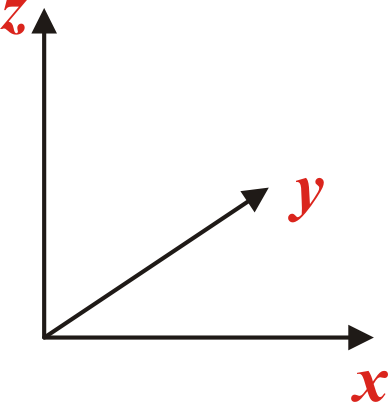
\includegraphics[width=3cm]{pics/cartesian.png}
 \end{center}
  \caption{Global cartesian coordinate system}
  \label{fig:globCart}
\end{figure}

\subsection{Local Polar}
In 2D, a polar coordinate system (see Fig. \ref{fig:locPolar}) can only be
defined in the x-y-plane. Each point is uniquely defined by its radial component
$r$ and the angle $\varphi$ in circumferential direction
\begin{equation}
 \vec{x} = \left(
\begin{array}{c}
r \\ \varphi \\
\end{array}
\right)
\end{equation}
In order to define a local polar coordinate system, one needs to specify the
origin of the coordinate system and also the radial direction where $\varphi =
0^\circ$. 
\newline
\noindent
The related section in the xml-file looks like
\begin{xmllisting}
<polar name="myPolar1">
  <origin x="0" y="0"/>
  <rAxis  x="1" y="0"/>
</polar>
 \end{xmllisting}
Note that the absolute length of the vector $\vec{r}_{(\varphi = 0)}$ defined by
\xel{rAxis} does not matter, as it gets normalized to 1.
\begin{figure}[ht]
 \begin{center}
   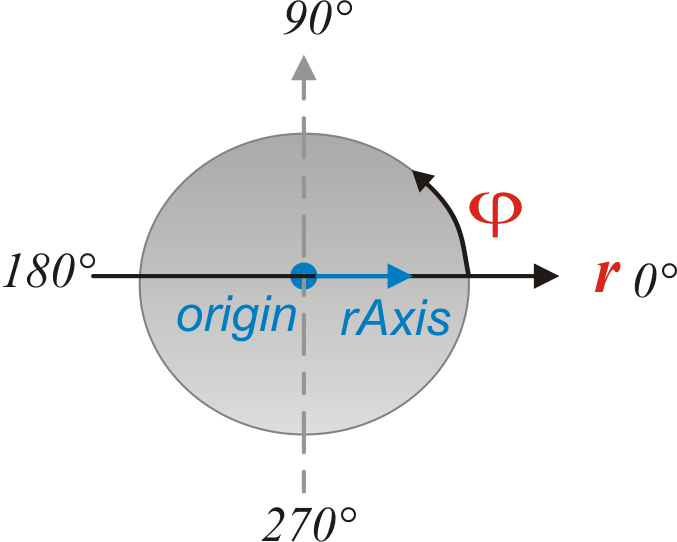
\includegraphics[width=5cm]{pics/polar.png}
 \end{center}
  \caption{Local polar coordinate system}
  \label{fig:locPolar}
\end{figure}

\subsection{Local Cylindrical}
In a 3D grid a cylindrical coordinate system is defined by its radial,
circumferential and axial direction ($z$-direction) (see Fig.
\ref{fig:locCylindric}
\begin{equation}
 \vec{x} = \left(
\begin{array}{c}
r \\ \varphi \\
z
\end{array}
\right)
\end{equation}
In order to define a cylindrical coordinate system, one needs to specify the
origin, the radial direction where $\vec{r}_{(\varphi = 0)}$ and the axial
$z$-direction.

\begin{xmllisting}
<cylindric name="myCylindrical1">
  <origin x="0" y="0" z="0"/>
  <zAxis  x="0" y="0" z="0"/>
  <rAxis  x="1" y="0" z="0"/>
</polar>
\end{xmllisting}
Similar to the polar coordinate system, the absolute length of the vectors
$\vec{r}_{(\varphi = 0)}$ and $\vec{z}$ does not matter, as they get normalized
to 1.

\begin{figure}[ht]
 \begin{center}
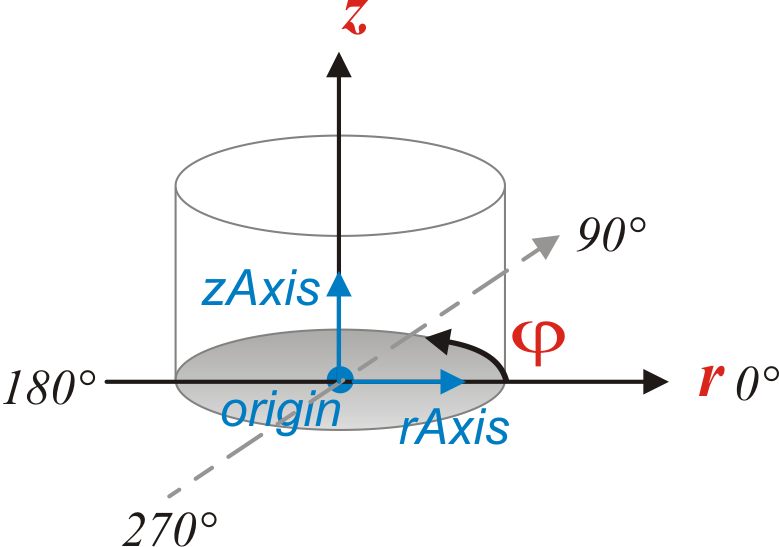
\includegraphics[width=6cm]{pics/cyl.png}   
 \end{center}
  \caption{Local cylindrical coordinate system}
  \label{fig:locCylindric}
\end{figure}

\newpage
\section{Material assignment}
\label{sec:materialAss}
A material has to be assigned for each region, as denoted in section
\ref{sec:geometricDef}. In addition there are several options which can be
defined for each region/material in addition.

\subsection{Material coordinate system}
\label{sec:materialCoordSys}
The material data (e.g. tensor of elasticity modulus) is defined in a separate
material local coordinate system, which is defined by the three axes $(1,2,3)$
as shown in Fig. \ref{fig:matCoordSys}.
\begin{figure}[ht]
\begin{center}
 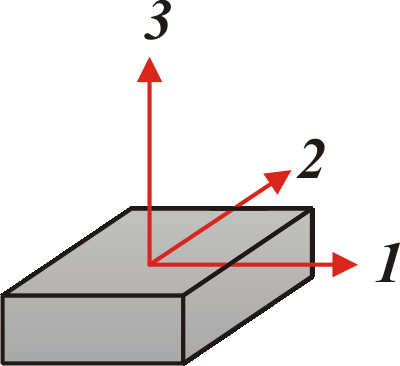
\includegraphics[width=3cm]{pics/matCoord.png}
\end{center}
\caption{Material coordinate system $(1,2,3)$}
  \label{fig:matCoordSys}
\end{figure}
If no further option is specified, the material coordinate directions $(1,2,3)$
get associated with the global cartesian direction $(x,y,z)$. 

In order to rotate the material coordinate system, one can specify three
rotation angles (\emph{Kardan angles})
\begin{equation}
\left( 
 \begin{array}{c}
 \alpha \\ \beta \\ \gamma 
 \end{array}
\right)
\end{equation}
These angles define three successive rotations around the three material axes
(see Fig. \ref{fig:matRotation}). This is done in three steps
\begin{enumerate}
 \item Rotation of $\alpha$ degrees around material direction 1 (= global
direction $x_0$)
 \item Rotation of $\beta$ degrees around material direction 2 (= global
direction $y_1$)
 \item Rotation of $\gamma$ degrees around material direction 3 (= global
direction $z_2$)
\end{enumerate}
The rotation can be specified for each region separately in the parameter file
by the three rotation angles $\alpha, \beta, \gamma$:
\begin{xmllisting}
  <domain>
    <region name="pzt" material="PZT-4">
      <matRotation alpha="-90" beta="0" gamma="-90"/>
    </region>
  </domain>
\end{xmllisting}
The previous example would e.g. first rotate the (material-) local $3$-direction
by $\alpha=-90^\circ$ around the local $1$-axis, so that it coincides with the
global $y$-direction. In a second step then the material is rotated around the
local $3$-axis by $\gamma=-90^\circ$, such that the local $2$-direction
coincides with the global $x$-direction. 
This is needed, if for example a plane simulation of a piezoelectric material
has to be performed, where the polarization is given in local $3$-direction,
whereas the geometric model assumes a polarization in $y$-direction. So in the
end, the material 23-plane coincides with the geometrical xy-plane.
\newline

{\bf NOTE:} In a 2D simulation (\myverb#<domain geometryType="plane/axi"/>#) the
rotation described above is always performed automatically by CFS++, until the
user gives another explicit rotation command. This is done to ensure that a
piezoelectric material is always poled in y-direction ( good old CAPA ...)!
\newline

Please note, that the positive direction of the angles is always defined in
counter-clockwise fashion around the corresponding axis
(\emph{right-hand-rule}). If the value of one rotation angle is $0$, it may be
omitted.

\begin{figure}[h!]
\begin{center}
 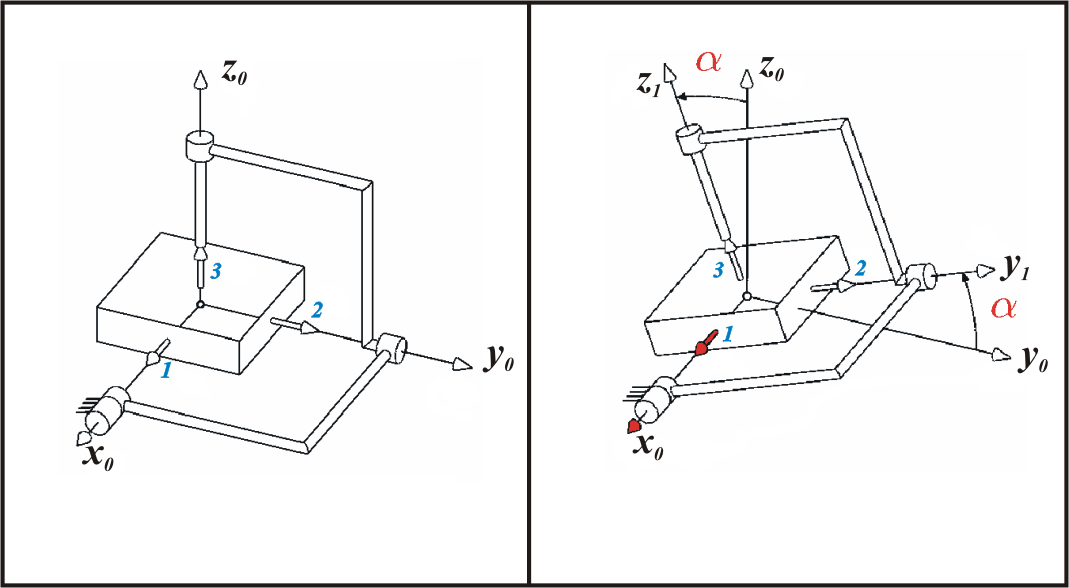
\includegraphics[width=13cm]{pics/rot1.png}
 % matCoord.png: 2228x588 pixel, 300dpi, 18.86x4.98 cm, bb=0 0 535 141
 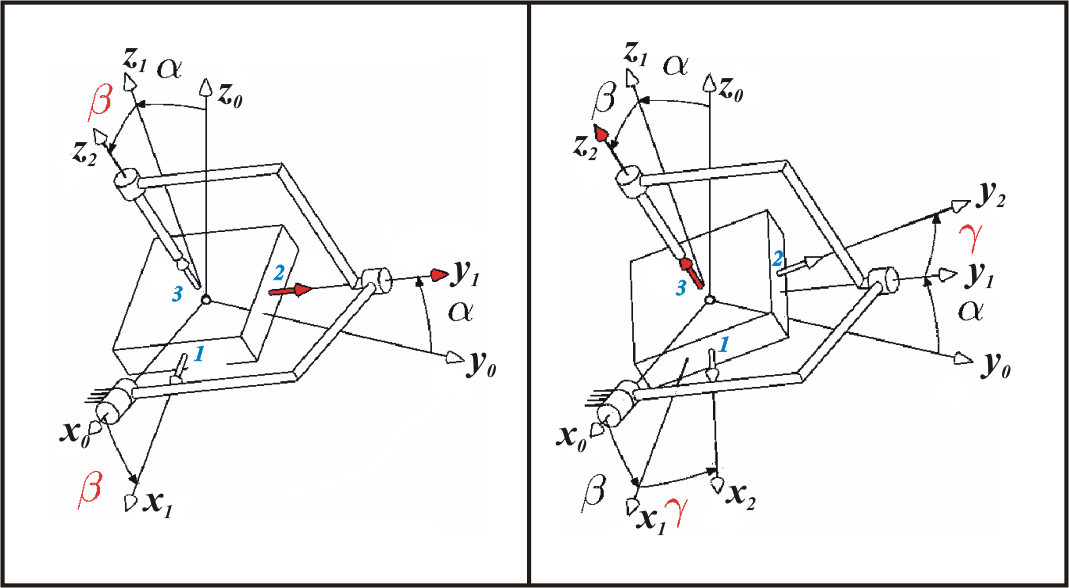
\includegraphics[width=13cm]{pics/rot2.png}
 % matCoord.png: 2228x588 pixel, 300dpi, 18.86x4.98 cm, bb=0 0 535 141
\end{center}
\caption{Rotation of material coordinate system (1,2,3) by Kardan angles
$(\alpha, \beta, \gamma)$}
  \label{fig:matRotation}
\end{figure}

\subsection{Rotated material coordinate systems}
A material can also be associated with a local coordinate system, as defined in
section \ref{sec:coordSys}. This allows one, e.g. to have a radially polarized
material in 2D (polar coordinate system) or in 3D (cylindrical coordinate
system). In this case, the material local directions $(1,2,3)$ are associated
with the global directions as defined in Table \ref{tb:matLocGlobAssoc}.
\begin{table}[h!]
\begin{center}
% use packages: array
\begin{tabular}{llll}
\toprule
 Material Direction & \multicolumn{3}{c}{Local Coordinate system} \\
 \cmidrule(r){2-4}
 & cartesian & polar & cylindrical \\
\midrule 
1 & x & r & r \\ 
2 & y & phi & phi \\ 
3 & z &  & z \\
\bottomrule 
\end{tabular}
\end{center}
\caption{Association of material directions $(1,2,3)$ with local coordinate
system directions}
\label{tb:matLocGlobAssoc}
\end{table}
In the parameter file, this can be defined by
\begin{xmllisting}
  <domain>
    <region name="pzt" material="PZT-4" refCoordSys="myPolar1"/>
  </domain>
\end{xmllisting}
Here the material PZT-4 is associated with a previously defined coordinate
system \xatv{myPolar1}.

It is also possible to rotate a material first - as defined in section
\ref{sec:materialCoordSys} - and then associate it with a local coordinate
system:
\begin{xmllisting}
  <domain>
    <region name="pzt" material="PZT-4" refCoordSys="midPoint">
      <matRotation beta="90"/>
    </region>
    <coordSys>
     <cylindric name="midPoint"> 
        <origin x="0" y="0" z="0"/>
        <zAxis  x="0" y="1" z="0"/>
        <rAxis  x="1" y="0" z="0"/>
      </cylindric>
    </coordSys>
  </domain>
\end{xmllisting}
In this example the following happens (see Fig. \ref{fig:matRotationExample}):
\begin{itemize}
 \item First, the material is rotated around the material local $2$-axis by
$\beta=90^\circ$, so that the local $3$-direction coincides with the global
$x$-direction.
\begin{equation}
\left( 
\begin{array}{c}
  1 \\ 2 \\ 3 
 \end{array}
\right)
\rightarrow
\left(
\begin{array}{c}
  -z \\ y \\ x 
 \end{array}
\right)
\end{equation}
\item Then the material gets associated with a cylindrical local coordinate
system, which radial direction coincides with the $x$-axis and which axial
direction is the $y$-axis.
\begin{equation}
\left( 
\begin{array}{c}
  x \\ y \\ z 
 \end{array}
\right)
\rightarrow
\left(
\begin{array}{c}
  r \\ z \\ -\varphi 
 \end{array}
\right)
\end{equation}

\end{itemize}

Putting both definitions together, the material axes $(1,2,3)$ are associated
with the cylindric components $(r,\varphi,z)$in the following way
\begin{equation}
\left( 
\begin{array}{c}
  1 \\ 2 \\ 3 
 \end{array}
\right)
\rightarrow
\left(
\begin{array}{c}
  \varphi \\ z \\ r 
 \end{array}
\right)
\end{equation}
The procedure is visualized in Fig. \ref{fig:matRotationExample}.
\begin{figure}[h!]
\begin{center}
 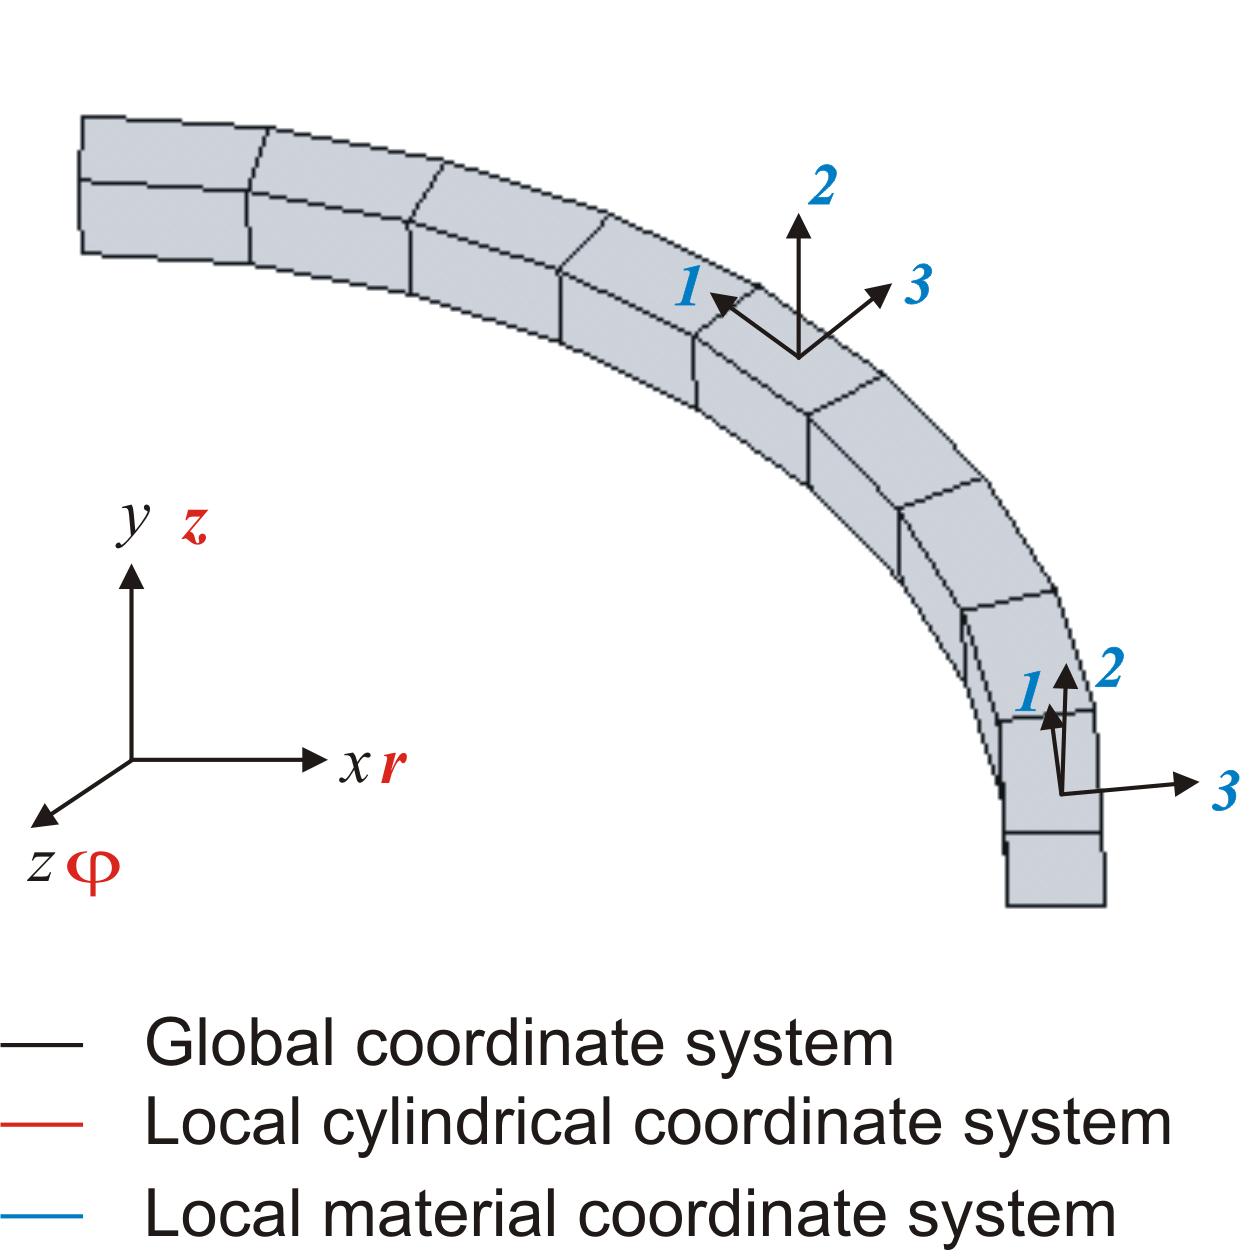
\includegraphics[width=8cm]{pics/cylExample.png}
\end{center}
\caption{Rotated material associated with a cylindrical coordinate system}
  \label{fig:matRotationExample}
\end{figure}


\section{Numerical Integration Rules}
The numerical integration of the finite elements is done via Gaussian
quadrature\footnote{See \emph{Higher-Order Finite Element Methods},
  Pavel Solin, Karel Segeth, Ivo Dolezel, 2004.}. Note that the integration
rules are theoretically exact for the given order and hence a too low order of
Ansatz-functions, a too coarse or deformed meshing cannot be compensated simply
by a higher integration order. Table \ref{tab:default_order} gives the default
order which should be sufficient for most simulations.

\begin{table}[ht]
\begin{center}
\begin{tabular}{lcccc}
\toprule
element & Ansatz-function & Gauss order & number of points \\
\midrule
line & 1 & 1 & 1\\
     & 2 & 2=3 & 2 \\
\midrule
triangle & 1 & 2 & 3 \\
         & 2 & 3 & 4 \\
\midrule
rectangle & 1 & 2=3 & 4 \\
          & 2 & 4=5 & 8 \\
\midrule
tetrahedron & 1 & 1 & 1 \\
         & 2 & 2 & 4 \\
\midrule
hexahedron & 1 & 4=5 & 14 \\
         & 2 & 4=5 & 14 \\
\bottomrule         
\end{tabular}
\caption{This are the default settings for numerical integration of elements via
Gaussian quadrature. Note that the integration rules for odd and even orders
coincide for line, rectangle and hexahedron elements.}
\label{tab:default_order}
\end{center}
\end{table}
 
One can optionally define a different integration rule in the following way:
\begin{xmllisting}
<integRules>
  <type>Gauss_standard</type>
  <order>5</order>
</integRules>
\end{xmllisting}

The setting is applied on all element types, even if they are not used in the simulation. If the requested integration rule is not known for an element, CFS uses a default setting and prints a warning message stating all available integration rules for that element. A typical usage is for rectangualar elements with quadratic ansatz functions, here second order integration is in most cases sufficient.

\begin{center}
\begin{tabular}{ll}
\toprule
integration type & description \\
\midrule
Gauss\_standard & The so called economical Gaussian quadrature rules. \\
Classic & The legacy implementation, not of general interest. \\
Lobatto & An alternative integration rule for 1D. \\
Chebyshev & An alternative integration rule for 1D. \\
\bottomrule
\end{tabular}
\end{center}

%%% Local Variables: 
%%% mode: latex
%%% TeX-master: "singlefields"
%%% End: 
